\section{Channel diagnostics}\label{app:diagnostics}

The prediction of the cost model was tested on a uniform sample of $2\times10^4$ points per system (Figure~\ref{fig:signal}). Channel B works when nontarget points with long transients converge spatially to the target. For Chua~II, the median distance $d(\alpha)$ decreases with the upper-set fraction $\alpha$ as $0.43\to0.19\to0.12$; for LE1, as $0.53\to0.22\to0.13$; for SE11, as $0.47\to0.19\to0.15$; and for D2, as $0.74\to0.60\to0.53$ (at $\alpha=0.2$, 0.04, and 0.008); the splitting gain here is 2.5--8.3 times. For the Jafari cycle ($0.99\to1.35$) and for D1 ($1.26\to1.38\to1.41$), $d(\alpha)$ grows, and there is no gain. At the same time, in D1, the fraction of the target in the upper sets grows: the regions of long trajectories are scattered, and there is no path to the target through them. The AUC of the coordinate $\xi$ alone (0.88--0.97 for all systems except the Jafari cycle, 0.61) does not separate these cases, whereas $d(\alpha)$ does; the asymptotic features, the Lyapunov exponent and the maximum norm, give AUC values of 0.50--0.74, except for the maximum norm on D1 (0.92), where the gate sets the amplitude of trajectories outside the ball. For the Huynh map, there is a gradient over only one decade ($d$ drops to 0.22 and grows again); at $p\approx0.009$, it barely pays back the initial sample and the levels.

\begin{figure}[tbhp]
\centering
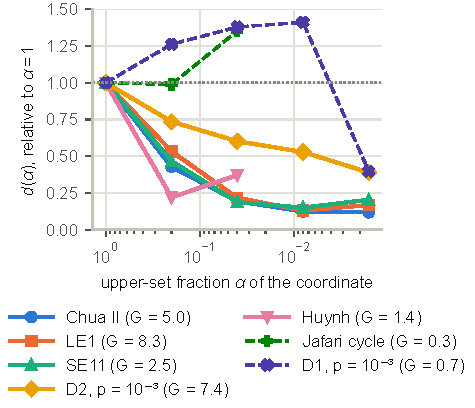
\includegraphics[width=0.62\textwidth]{figures/fig26_signal_curves.pdf}
\caption{Diagnostics of channel B from a uniform sample: the median distance from nontarget points of the upper set of the coordinate $\xi$ to the target (relative to its value for the whole sample, $\alpha=1$) versus the fraction $\alpha$, which decreases to the right. The legend gives the splitting gain $G_{0.9}$. A decreasing $d(\alpha)$ (solid: Chua~II, LE1, SE11, D2) comes with a splitting gain (Tables~\ref{tab:gains} and \ref{tab:scaling}), and an increasing one (dashed: Jafari cycle, D1) with its absence; for the Huynh map, $d(\alpha)$ decreases over one decade only, and the gain is small.}
\label{fig:signal}
\end{figure}

